\documentclass{article}

\usepackage{tikz}
\usepackage{verbatim}
\usepackage{parskip}
\usepackage{amsthm}
\usepackage{xpatch}
\usepackage{amsmath}
\usepackage{graphicx}

\graphicspath{ {./img/} }

\setlength\parindent{0pt}

\newtheorem{definicija}{Definicija}[subsection]
\newtheorem{lema}{Lema}[subsection]
\newtheorem{izrek}{Izrek}[subsection]
\newtheorem{trditev}{Trditev}[subsection]
\newtheorem{posledica}{Posledica}[subsection]
\newtheorem{domneva}{Domneva}[subsection]
\newtheorem{primer}{Primer}[subsection]
\newtheorem{opomba}{Opomba}[subsection]

\makeatletter
\xpatchcmd{\@thm}{\thm@headpunct{.}}{\thm@headpunct{:}}{}{}
\makeatother

\begin{document}
\pagestyle{empty}

\begin{comment}
definitions
\end{comment}

%%%%%%%%%%%%%%%%%%%%%%%%%%%%%%%%%%%%%%%%%%%%%%%%%%%%%%%%%%%%%%%%%
\section{ Obseg in ploscina (enačbe) }

\subsection{ Štirikotnik }
$ o = a + b + c + d$

\subsection{ Kvadrat }
$ o = 4 \cdot a $ \\
$ p = a \cdot a = a ^ 2$


\subsection{ Pravokotnik }
$ o = 2 \cdot a + 2 \cdot b $ \\
$ p = a \cdot b$

\subsection{ Trikotniki }
$ o = a + b + c $ \\
$ p = \frac{a \cdot v_a}{2} = \frac{b \cdot v_b}{2} = \frac{c \cdot v_c}{2} $

\begin{figure}[h]
    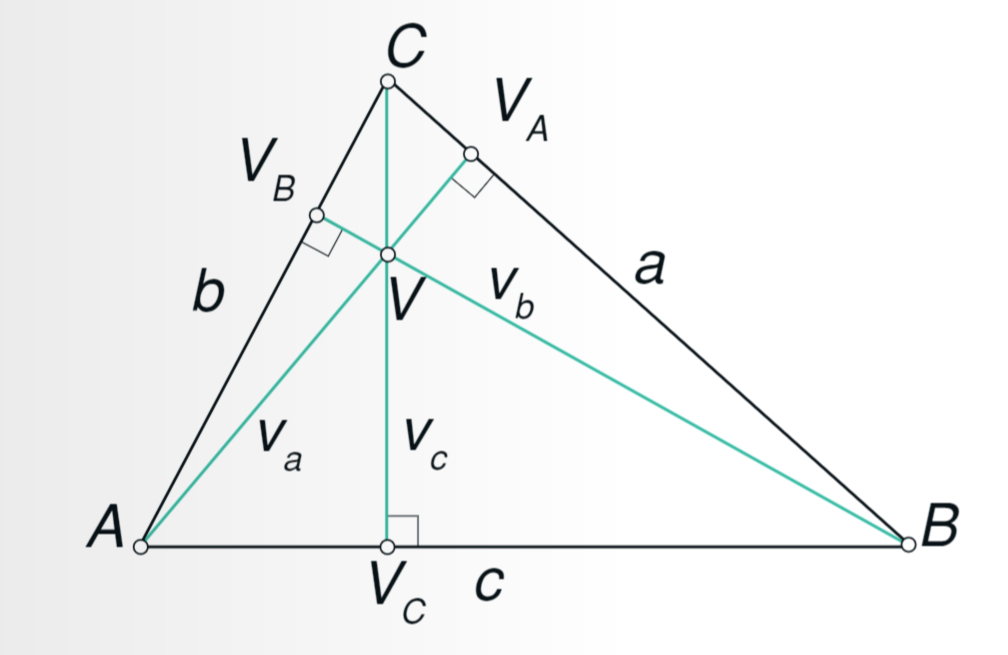
\includegraphics[width=0.4\linewidth]{trikotnik.png}
    % \centering
    % \caption{Izračun ploščine s preoblikovanjem lika v pravokotnik.}
\end{figure}

\subsection{ Paralelogram }
$ o = 2 \cdot a + 2 \cdot b $ \\
$ p = a \cdot v_a \quad \text{ali} \quad p = b \cdot v_b $

\begin{figure}[h]
    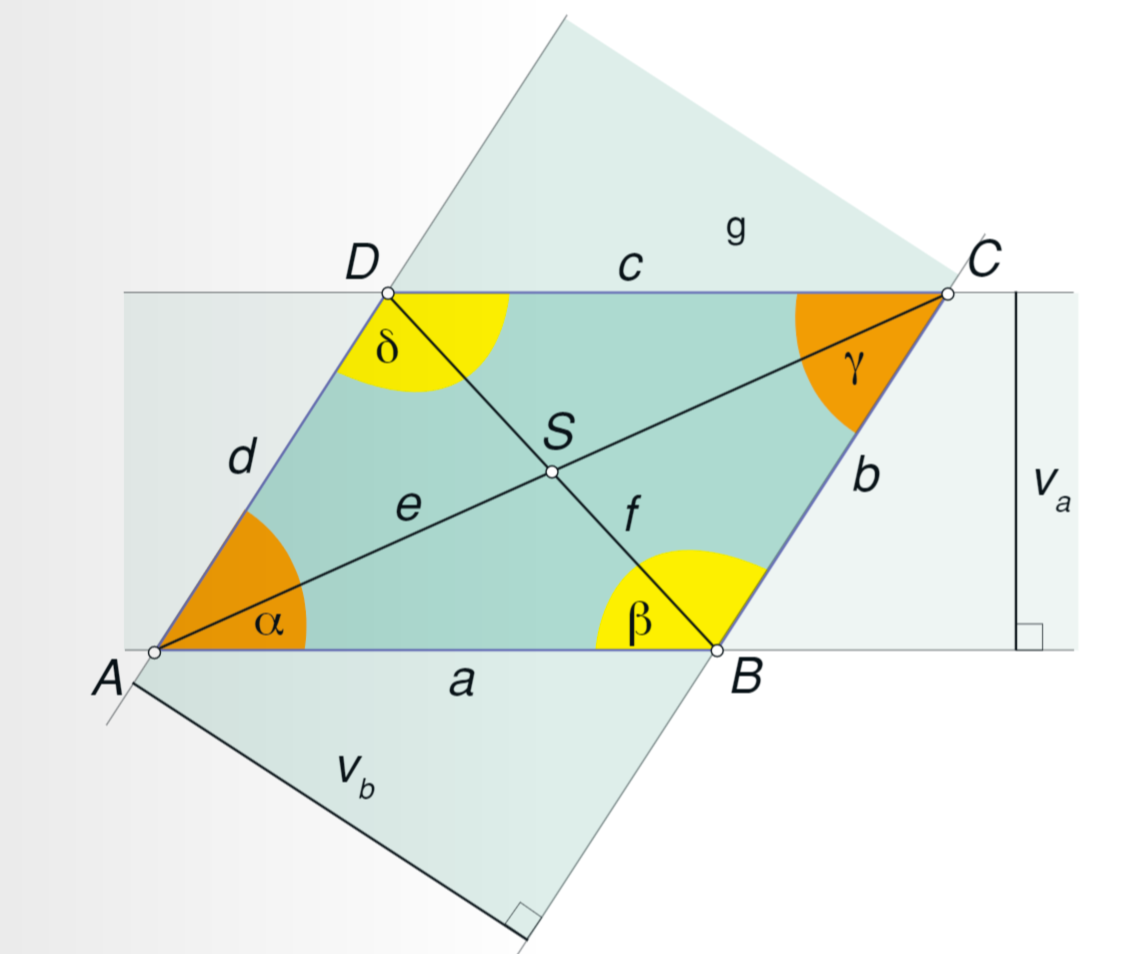
\includegraphics[width=0.4\linewidth]{paralelogram.png}
    % \centering
    % \caption{Izračun ploščine s preoblikovanjem lika v pravokotnik.}
\end{figure}

\subsection{ Romb (enakostranični paralelogram) }
$ o = 4 \cdot a $ \\
$p = a \cdot v_a $


\subsection{ Deltoid, romb, kvadrat }
Štirikotniki s pravokotnimi diagonalami (deltoid, romb, kvadrat,...). \\
$ p = \frac{e \cdot f}{2} $ 
\begin{figure}[h]
    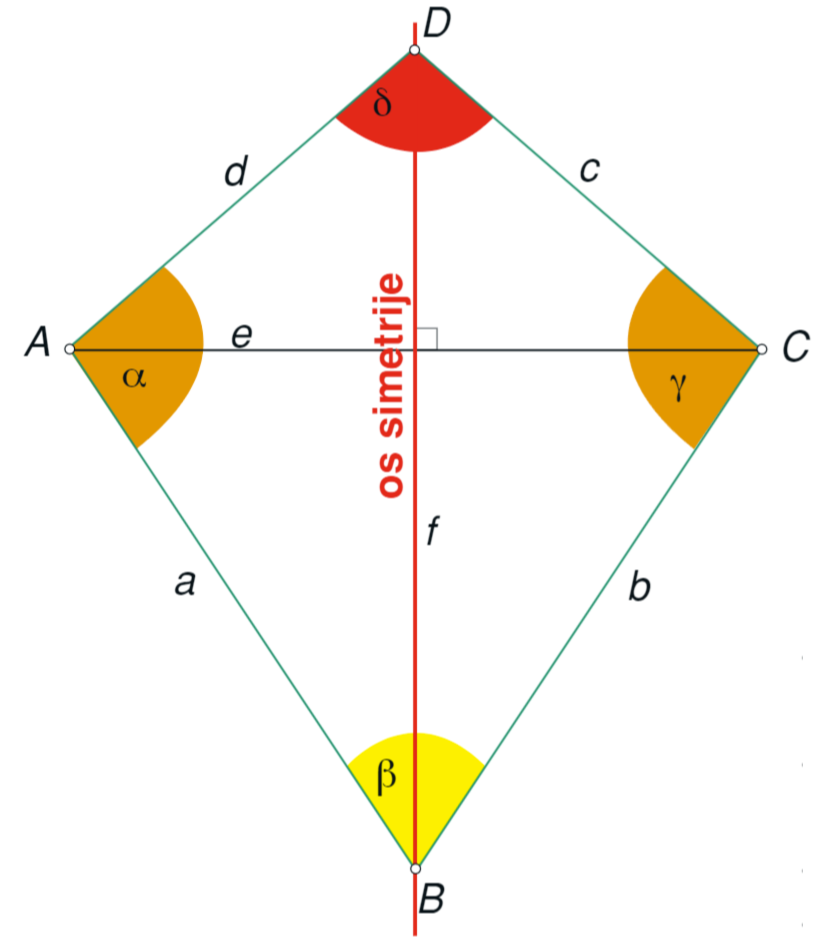
\includegraphics[width=0.4\linewidth]{deltoid.png}
    % \centering
    % \caption{Izračun ploščine s preoblikovanjem lika v pravokotnik.}
\end{figure}

\subsection{ Trapez }
$s = \frac{a + c}{2}$ \\
$ p = s \cdot v =  \frac{a + c}{2} \cdot v$

\begin{figure}[h]
    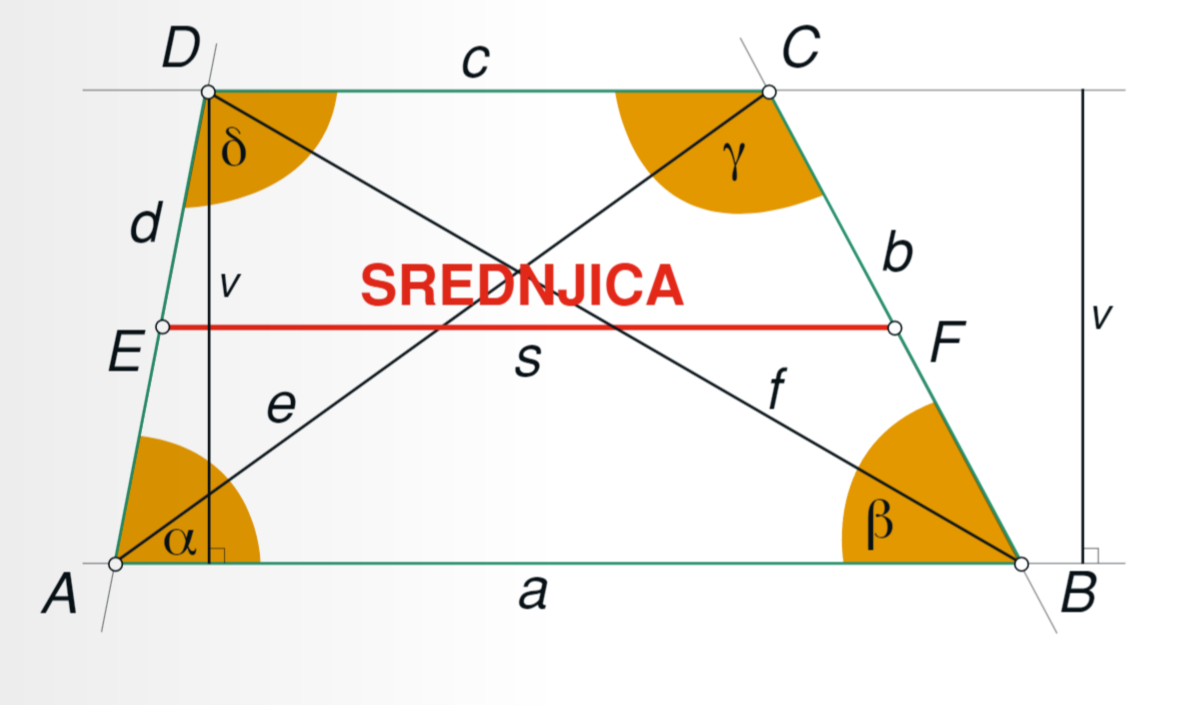
\includegraphics[width=0.4\linewidth]{trapez.png}
    % \centering
    % \caption{Izračun ploščine s preoblikovanjem lika v pravokotnik.}
\end{figure}


\end{document}